% 04_p2_dimensional.tex —— P2 无量纲化与解析关系
\section{Problem 2: Dimensional Analysis and the $R(t_s)$ Relation}

\subsection{Scaling}

The pressure redistribution after shut-in is governed by the hydraulic
diffusivity $D=k/(\phi\mu c_t)$. We use the diffusion length as the length
scale and the soak time as the time scale:
\begin{equation}
L_c=\sqrt{D_0t_s},\qquad t_c=t_s,\qquad
\Delta p_c=p_{inj}-p_0,\qquad C_c=C_{n,inj},
\label{eq:scales}
\end{equation}
and define
\begin{equation}
x_D=\frac{x}{L_c},\qquad t_D=\frac{t}{t_s},\qquad
p_D=\frac{p-p_0}{p_{inj}-p_0},\qquad C_D=\frac{C_n}{C_{n,inj}} .
\label{eq:dimless}
\end{equation}
With these variables the diffusion equation becomes
$\partial p_D/\partial t_D=\partial^2p_D/\partial x_D^2$, so the
dimensionless radius is a function of the dimensionless initial profile and of
the threshold ratio only.

\subsection{Dimensionless Groups}

\begin{table}[h!t]
\centering
\caption{Dimensionless controlling groups and their magnitudes for Case~3
($p_0=48$~MPa, $\sigma_h=48$~MPa, $k_{m0}=0.5$~mD, $\phi_0=0.13$).}
\label{tbl:pi_groups}
\small
\begin{tabular}{clll}
\toprule[1.5pt]
Group & Definition & Physical meaning & Magnitude\\
\midrule[1pt]
$\Pi_0$ & $R/\sqrt{D_0t_s}$ & dimensionless stimulation radius & $0.4$--$1.5$\\
$P$ & $(p_{inj}-p_0)/p_0$ & injection intensity & $0.10$\\
$\Gamma$ & $\gamma_k p_0$ & stress-sensitivity strength & $0.96$\\
$C_\phi$ & $c_\phi p_0$ & pressure sensitivity of porosity & $0.024$\\
$\Lambda$ & $\alpha(p_{inj}-p_0)/\sigma_h$ & Biot coupling strength & $0.076$\\
$\Delta_d$ & $\beta_d\varepsilon_d$ & damage-initiation strength & $0.48$\\
$K_a$ & $(1-\phi)\rho_rK_d/(\phi S_w)$ & adsorption vs.\ mobile aqueous inventory
& $6\times10^{2}$\\
$A_\sigma$ & $a_\sigma C_{n,inj}$ & IFT-reduction amplitude & $0.30$\\
$A_\theta$ & $a_\theta C_{n,inj}$ (rad) & contact-angle change amplitude & $0.26$\\
$Pe$ & $vL/D$ & advection--diffusion ratio & $7\times10^{-4}$\\
\bottomrule[1.5pt]
\end{tabular}
\end{table}

The very large $K_a$ shows that adsorption dominates the aqueous inventory:
almost all injected nanoparticles are retained near the fracture, and the
aqueous concentration is controlled by the local sorption equilibrium rather
than by advection. The small $Pe$ confirms that molecular diffusion, not
advection, sets the nano front during soaking.

\subsection{Approximate Analytical Relation $R(t_s)$}

Let $t_s=0$ denote the end of injection and let
$u_0(x)=p(x,0)-p_0$ be the pressure disturbance at that instant. During
shut-in the fracture face is impermeable, so the semi-infinite problem has a
zero-flux condition at $x=0$. The mirror-image heat kernel gives, for a
step-like initial disturbance $u_0\simeq A\,\mathbf 1_{[0,a]}(x)$,
\begin{equation}
u(x,t_s)=\frac{A}{2}\left[
\operatorname{erf}\!\left(\frac{a+x}{2\sqrt{Dt_s}}\right)
+\operatorname{erf}\!\left(\frac{a-x}{2\sqrt{Dt_s}}\right)\right].
\label{eq:kernel}
\end{equation}
The two parameters are read directly from the injection-end profile:
$A=u_0(0)$ and $a=A^{-1}\int_0^L u_0(x)\,dx$. The stimulation radius is the
farthest non-negative root of
\begin{equation}
u(R,t_s)=0.05\,p_0 .
\label{eq:threshold}
\end{equation}
If $u(0,t_s)<0.05p_0$, the face itself is below the threshold and we set
$R=0$; no extrapolation is attempted. For a sustained constant-pressure step,
the classical result
\begin{equation}
R=2\sqrt{Dt_s}\,\operatorname{erfc}^{-1}\!\left(
\frac{0.05p_0}{p_{inj}-p_0}\right)
\label{eq:erfc}
\end{equation}
is retained as a check \cite{p2-01}.

\paragraph{Numerical check.}
Using the three-phase model of Problem~1 with $N_f=10$, $L=40$~m and 100
cells, the injection-end profile gives $A=4.82$~MPa,
$a=19.05$~m at $q_{inj}=300$~m$^3$/d, and $A=8.14$~MPa, $a=15.6$~m at
$q_{inj}=800$~m$^3$/d. The numerical shut-in radius and the kernel prediction
are compared in Table~\ref{tbl:p2_check}.

\begin{table}[h!t]
\centering
\caption{Pressure-threshold radius during shut-in: three-phase simulation
($R_{num}$) versus the mirror-kernel solution ($R_{semi}$).}
\label{tbl:p2_check}
\small
\begin{tabular}{cccc}
\toprule[1.5pt]
$q_{inj}$ (m$^3$/d) & $t_s$ (d) & $R_{num}$ (m) & $R_{semi}$ (m)\\
\midrule[1pt]
300 & 1 & 18.08 & 18.58\\
300 & 2 & 14.80 & 14.00\\
300 & 3 & 8.48 & 0\\
300 & 4 & 0 & 0\\
800 & 1 & 23.94 & 24.39\\
800 & 2 & 23.38 & 25.74\\
800 & 3 & 21.24 & 24.54\\
800 & 5 & 13.21 & 15.33\\
800 & 6 & 4.32 & 0\\
800 & 8 & 0 & 0\\
\bottomrule[1.5pt]
\end{tabular}
\end{table}

The kernel reproduces the numerical radius while both are non-zero, but it
reaches zero earlier. The same happens for a constant-coefficient finite-domain
solution with the same initial profile. Consequently we do not report a
relative error for the zero-crossing region; the semi-infinite kernel is used
for scaling and trend, while the quantitative radius is taken from the
three-phase forward model. For the two cases in Table~\ref{tbl:p2_check}, the
5\% radius falls below the threshold at $3$--$4$~d for
$q_{inj}=300$~m$^3$/d and at $6$--$8$~d for $q_{inj}=800$~m$^3$/d, consistent
between 100 and 200 cells.

\paragraph{Dimensionless master curve.}
With $\tau=Dt_s/a^2$, $r=R/a$ and $\mathcal A=A/(0.05p_0)$, the kernel
collapses onto a one-parameter family. Table~\ref{tbl:master} and
Figure~\ref{fig:p2_master} show the result. For $\mathcal A\lesssim2$ the
radius contracts monotonically; for $\mathcal A\gtrsim4$ it first expands and
then contracts; for $\mathcal A\approx17$ it survives beyond 60~d. The
injection strength therefore controls whether a pressure-based stimulation
radius exists at all during a long soak.

\begin{table}[h!t]
\centering
\caption{Dimensionless radius $r=R/a$ at $\tau=0.1,1,10,30$ for several
$\mathcal A=A/(0.05p_0)$.}
\label{tbl:master}
\small
\begin{tabular}{ccccc}
\toprule[1.5pt]
$\mathcal A$ & $\tau=0.1$ & $\tau=1$ & $\tau=10$ & $\tau=30$\\
\midrule[1pt]
2.08 & 1.022 & 0.613 & 0 & 0\\
4.17 & 1.316 & 1.912 & 0 & 0\\
8.33 & 1.525 & 2.625 & 3.972 & 0\\
16.67 & 1.695 & 3.181 & 6.633 & 8.056\\
\bottomrule[1.5pt]
\end{tabular}
\end{table}

\begin{figure}[h!t]
\centering
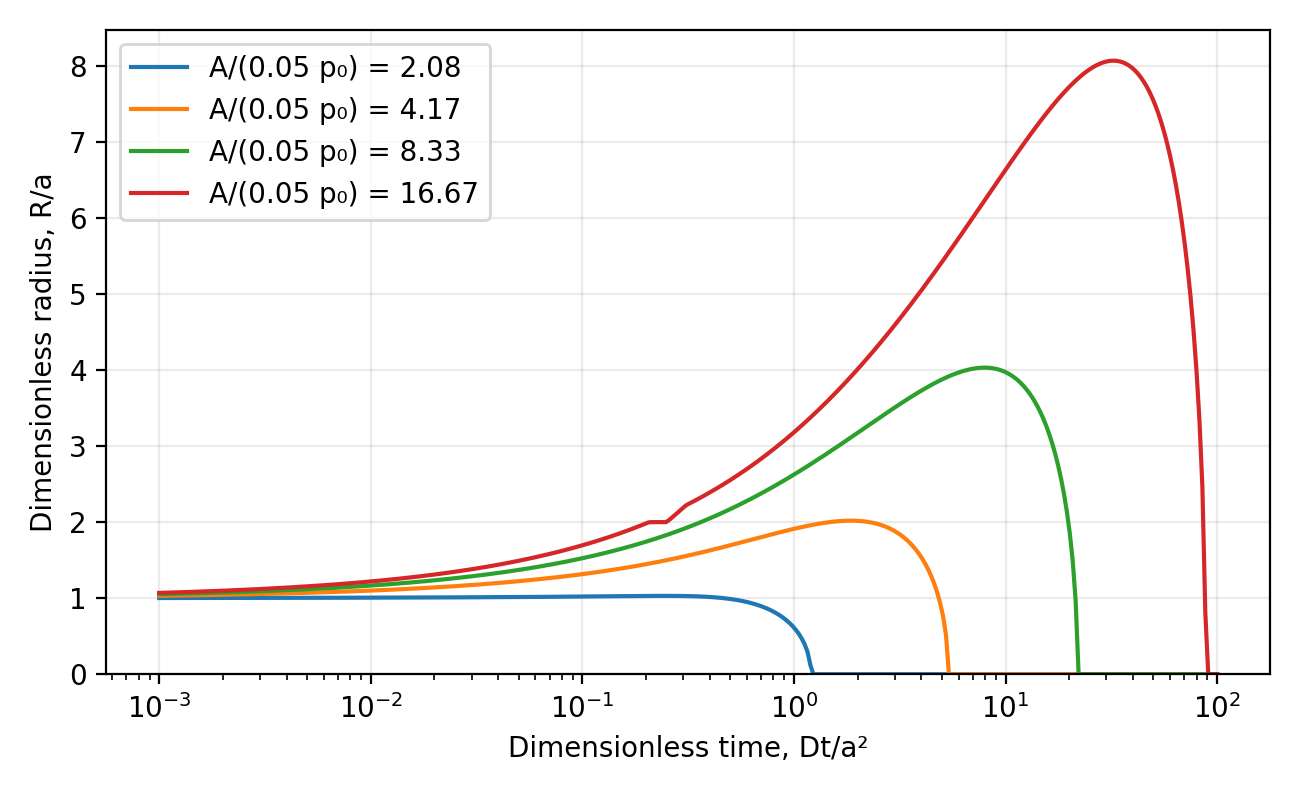
\includegraphics[width=0.62\textwidth]{p2_master}
\caption{Pressure-based stimulation radius under shut-in for several injection
strengths.}
\label{fig:p2_master}
\end{figure}

\subsection{Which Groups Matter, and Why the Soak-Time Sign Is Ambiguous}

The sensitivity of $R(t_s)$ is controlled mainly by $\Gamma$ and $P$.
Stress sensitivity changes the effective diffusivity during injection and
production, while $P$ sets the initial amplitude and therefore the
$\mathcal A$ that decides expansion versus contraction. $C_\phi$ and $\Lambda$
are secondary; $\Delta_d$ is inactive in the nominal range because the
compressive strain is below the damage threshold. The adsorption group $K_a$
does not affect the pressure radius, but it controls the nano front and
therefore the material-based radius.

This separation explains an apparent contradiction in the literature. Studies
that fix the total operation window report a weak negative correlation between
soak time and cumulative oil, because a longer soak consumes production time
\cite{p1-03}. In the present problem the production period is fixed at 360~d
after soaking; a longer soak does not consume production time, and its benefit
saturates as the material fronts slow down. The sign of the soak-time effect is
thus a property of the chosen time budget, not a universal physical law.

The four radius definitions of the problem statement differ by one to two
orders of magnitude. The pressure disturbance reaches tens of metres but
decays within days; the CO$_2$ and nano fronts move at sub-metre to metre
scales but persist; the damage radius is confined to the near-fracture zone.
For the Case~3 baseline the nano radius at 0.01~wt\% is about $0.15$~m with
the tabulated $K_d$ in m$^3$/kg, and about $0.52$~m if $K_d$ is interpreted
in L/kg; both values are grid-dependent and are reported with their mesh
refinement. The pressure radius is therefore not the limiting factor for a
long soak: the material fronts and the economics are.
